\chapter{Problem description}
\section{The necessity of a distributed system for collaborative science}
Nowadays, computers play an essential role in scientific research. For most scientists, a desktop machine is enough to store and process the data they work with, but a considerable amount of them need supercomputers to be able to deal with more complex problems \cite{computing-in-science}.

Supercomputers are expensive, and price ranges vary widely depending on the computational capacities of the system; For example, a supercomputer with a power of 40 TFLOPS like \textit{Alhambra}, the supercomputer at the \textit{University of Granada}, costs around \$670,000\cite{ideal-alhambra}. A supercomputer leading the list Top500,  like the one from \textit{Oak Ridge National Laboratory}, with 200 PetaFLOPS manufactured by IBM costs \$200 million\cite{oak-ridge}. Hence having access to one of these machines is not common.

Distributed systems are an attractive alternative to supercomputers. A distributed system can be defined as a set of independent machines that interact with each other, cooperating to achieve a common objective. Even though this approach is much cheaper than using a supercomputer, an important investment is required in order to buy and set up these machines.

In 2002, the \textit{University of California, Berkeley} addressed the problem described above by developing \textit{BOINC}\cite{boinc-website}, a platform for volunteer computing where users can contribute to different scientific projects with their computers or smart-phones. At the moment this chapter was written, the platform has achieved a power of over 27 PetaFLOPS in the last twenty-four hours by using 563,506 computers provided by 142,911 volunteers.

Even though \textit{BOINC} is a successful example of how volunteer computing is possible and what it can achieve, it still has room for improvement that this project aims to provide. 

On the one hand, a user willing to volunteer on \textit{BOINC} needs to download and set up his own machine in order to start collaborating with a project: non-tech-savvy users can struggle with this and may give up soon. This project addresses this problem by providing users a way to collaborate where they do not need to install anything apart from a web browser. Since most (if not all) consumer-oriented operative systems such as \textit{Ubuntu}, \textit{Mac OSX} or \textit{Windows} come with a web-browser installed out of the box, this platform provides a zero-installation method for volunteer computing.

On the other hand, \textit{BOINC} uses a Client-Server architecture where user's machines communicate with a centralized server that assigns them tasks. This centralized approach has a scalability problem where in case that the number of volunteers increases extremely or the amount of requests per user is high enough, the central server will not be able to handle the number of requests made by a user and therefore the performance of the system will reach its limit. This approach makes the system to have a single point of failure as well; if the central server goes down, users will not be able to work towards the common objective since they cannot communicate with each other, and therefore the whole experiment will be paused until the central server goes alive again.  

By using a decentralized architecture where nodes that satisfy certain criteria (detailed in later chapters) act as coordinators of the system, this project aims to provide better scalability and fault-tolerance than BOINC. 


\section{Evolutionary Algorithms}
Evolutionary Algorithms are metaheuristic optimization algorithms that take natural evolution as an inspiration to solve problems. They apply bio-inspired operations known as \textit{genetic operators} over a set of solutions to the problem called \textit{population}. Each solution inside the \textit{population} is known as \textit{chromosome} and has a \textit{fitness} value based on the quality of the solution itself. A \textit{chromosome} is made of \textit{genes}, these genes are specific characteristics of a solution representation. 
 
The simulation of this natural process is a probabilistic optimization technique that frequently achieves better results than other classic methods of solving hard problems. \cite{galist}. 

An overview of the implementation of this algorithm consists of the following steps

\begin{enumerate}
    \item \textbf{Initialization:} create a population with randomly generated chromosomes, and evaluate the fitness of each one.
    
    \item Until an specified termination condition is met, apply the following genetic operators over the population:
    
    \begin{enumerate}
        \item \textbf{\textit{Selection}:} pick which chromosomes from the population will reproduce, in other words, the \textit{crossover} operator will be applied. We should guarantee that the best chromosomes in the population have higher likelihood to be selected, while still giving the opportunity to chromosomes with less quality to reproduce.
    
        \item \textbf{\textit{Crossover}:} given two chromosomes, this operator will generate two or more new solutions that will inherit genes from both parents but will be different from them. These new solutions are known as \textit{Offsprings}.
        
        \item \textbf{\textit{Mutation}:} with a given probability, choose chromosomes to modify some of their genes.
        
        \item \textbf{\textit{Evaluation}:} evaluate the fitness of each chromosome in the population.
        
        \item \textbf{\textit{Replacement}:} replace the original population with the new one, following a given criteria. 
        
    \end{enumerate}     
\end{enumerate}

\begin{figure}[h!]
\centering
    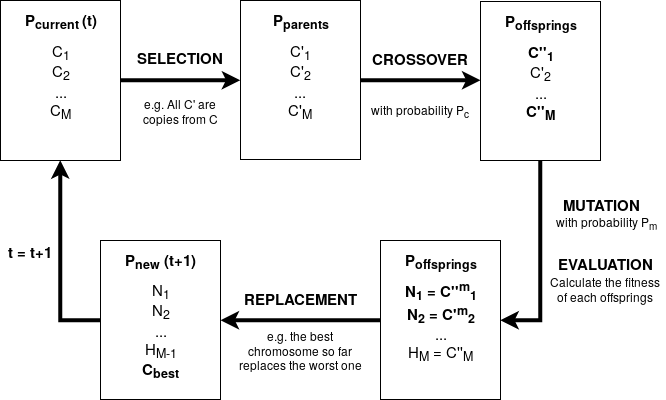
\includegraphics[width=\linewidth]{assets/images/EA_diagram.png}
    \caption{Overview of all genetic operators for a Evolutionary Algorithm}
    \label{fig:EA_diagram}
\end{figure}

To find good solutions with this algorithm we have to keep a good balance between exploitation and diversification. 

On the one hand, the selection, crossover and replacement operators focus on the exploitation of solutions with a promising fitness value in order to optimize solutions within a specific region of the search space. 

On the other hand, mutation and initialization diversify by generating rather different solutions from the existing ones; by doing so, the algorithm is able to explore new regions of the search space as well as avoiding getting stuck in local optima.

\section{Distributed Systems}
\begin{quotation}
\textit{A distributed system is a collection of independent computers that appears to its users as a single coherent system.}
\end{quotation}

\begin{figure}[h!]
\centering
    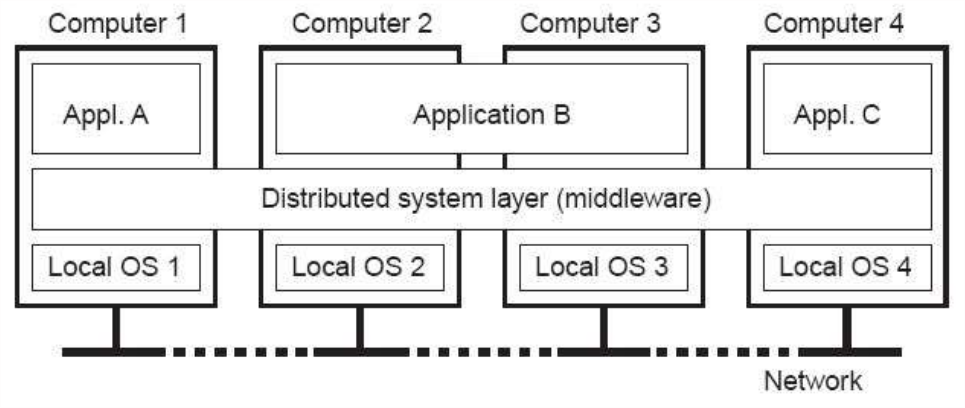
\includegraphics[scale=0.3]{assets/images/distributed-system_diagram.png}
    \caption{Distributed System from a user perspective}
    \label{fig:distributed_system}
\end{figure}

This collection of computers working as one needs to communicate, sharing information with each other in order to work towards the same objective. This exchange of communication can happen either by using shared memory or message passing.

Shared memory stands for memory that can be accessed concurrently by multiple programs. It is the fastest alternative but has two important disadvantages. The first one is that this alternative is expensive and does not scale well; it needs from these programs to be running within the same machine or at least be running in different machines that can share a common piece of hardware that stores the memory they share. The second main disadvantage of shared memory is that it is error prone; since multiple programs can access the same memory space, race conditions are likely to arise.

\begin{figure}[h!]
\centering
    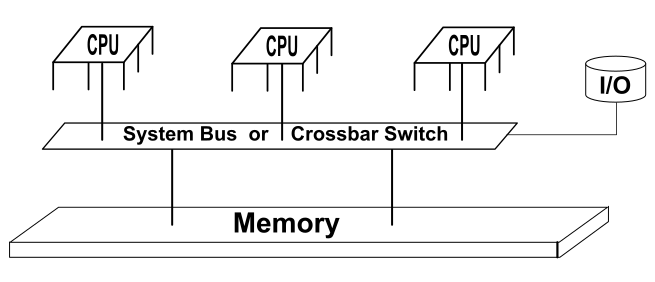
\includegraphics[scale=0.6]{assets/images/shared_memory.png}
    \caption{Shared memory system of three processors}
    \label{fig:shared_memory}
\end{figure}

Message passing is a method used to request behavior on a remote computer by sending an object containing enough information to select and run the appropriate code on the remote computer. this message passing can be synchronous if the requesting machine waits for the remote one to finish with the requested behavior, or asynchronous if it keeps busy on a different task. While synchronous systems are conceptually less complex, asynchronous ones usually achieve better performance.

Although this last approach comes with an overhead penalty due to data copying and delivery across machines, it is the best scaling one since interacting machines do not need to be close to each other to exchange information. Furthermore, because data sharing is explicit in message passing, there is less chance for error.





\section{Technosocial Systems}
